\documentclass{beamer}
\usetheme[
    block=fill,         % ブロックに背景をつける
    progressbar=foot,   % 各スライドの下にプログレスバー
    numbering=fraction  % 合計ページ数を表示
]{metropolis}           % Use metropolis theme

\usepackage{luatexja}% 日本語したい
\usepackage[ipaex]{luatexja-preset}% IPAexフォントしたい
\renewcommand{\kanjifamilydefault}{\gtdefault}% 既定をゴシック体に

\usepackage{float}
\usepackage{booktabs}
\usepackage{ascmac}
\usepackage{fancybox}
\usepackage{amsmath}
\usepackage{mathtools}
\usepackage{tikz}
\usetikzlibrary {arrows.meta}
\usetikzlibrary {bending}
\usepackage{graphicx,xcolor}
\usepackage{listings}
\lstset{
    frame=single,
    basicstyle=\tiny\ttfamily,
    tabsize=4
}

\title{進捗報告}
\date{\today}
\author{水野泰旭}
\institute{弘前大学理工学部電子情報工学科4年}
\subject{学習率による正解率向上}
\begin{document}
  \maketitle
  
\begin{frame}{目次}
    \tableofcontents
  \end{frame}

  \begin{frame}
    \section{k分割交差検証}
  \end{frame}

  \begin{frame}[fragile]{コードの修正}
    \begin{lstlisting}[language=Python, caption=kseparate\_train.py, label=cd:keseparate_train.py]
      k = 10
      n = len(images) // k
      label_size = len(set(labels))
      validation_scores = []
      for fold in range(k):
        print("The fold is :", fold)
        # SEPARATE TRAIN DATA
        validation_images = images[n * fold: n * (fold + 1)]
        validation_labels = labels[n * fold: n * (fold + 1)]
        train_images = np.concatenate([images[:n * fold], images[n * (fold + 1):]])
        train_labels = np.concatenate([labels[:n * fold], labels[n * (fold + 1):]])
      \end{lstlisting}
  \end{frame}

  \begin{frame}
    \begin{table}[H]
      \centering
      \caption{k分割交差検証結果(比率は無視)}
      \begin{tabular}{crr}
        \toprule
        fold & loss & accuracy \\
        \midrule
        1 & 0.2004694938659668 & 0.9520807266235352 \\
        2 & 0.0869437754154205 & 0.9747793078422546 \\
        3 & 0.1595330983400344 & 0.9697352051734924 \\
        4 & 0.1649435311555862 & 0.9546027779579163 \\ 
        5 & 0.1361409425735473 & 0.9596469402313232 \\
        6 & 0.1505440622568130 & 0.9533417224884033 \\
        7 & 0.1733103841543197 & 0.9508196711540222 \\
        8 & 0.2493898719549179 & 0.9407314062118530 \\
        9 & 0.1259648948907852 & 0.9672130942344666 \\
        10 & 0.1510167270898819 & 0.9697352051734924 \\
        \midrule
        average & 0.1598256722092628 & 0.9592686057090759 \\
        \bottomrule
      \end{tabular}
    \end{table}
  \end{frame}
  
  \begin{frame}{考察}
    \begin{itemize}
      \item 配列をシャッフルしてk個に分割したため、訓練データと検証データのラベルの比率が毎回バラバラになっているため、結果が正確とは言えない\mbox{}\\ $\rightarrow$sklearnを用いて、訓練データと検証データのラベルの比率を揃える
    \end{itemize}
  \end{frame}

  \begin{frame}
    \section{混同行列のヒートマップ}
  \end{frame}

  \begin{frame}{学習の様子}
    Test Accuracy: 0.9699519276618958
    \begin{figure}[H]
      \centering
      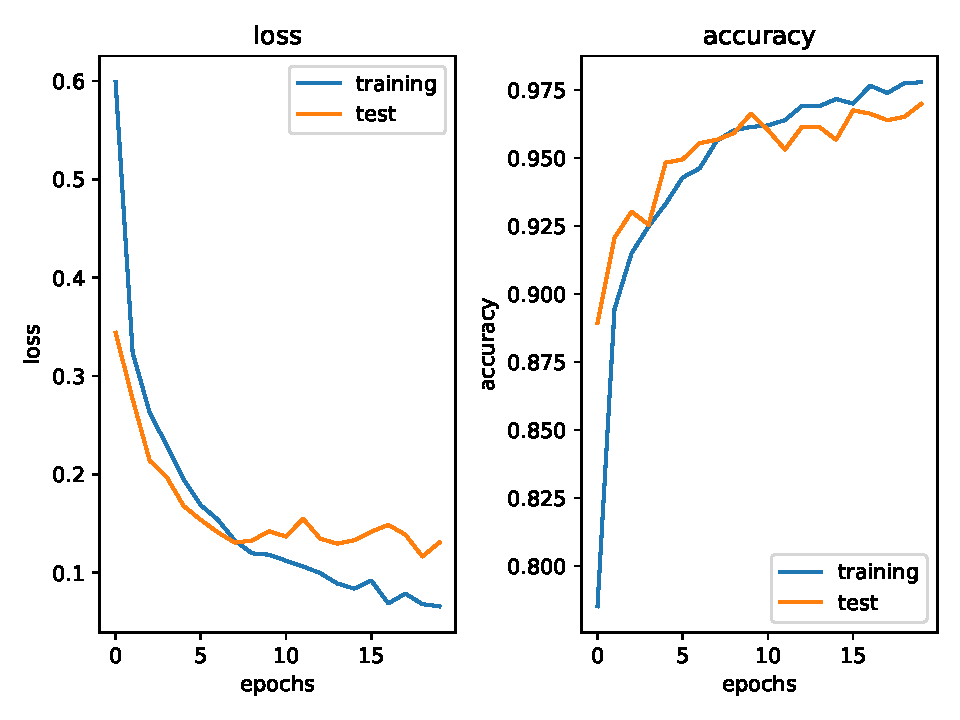
\includegraphics[keepaspectratio, scale=0.5]{images/deep_conv.pdf}
    \end{figure}
  \end{frame}

  \begin{frame}{混同行列(割合)のヒートマップ\footnote{縦軸が正解ラベル、横軸が予測ラベル}}
    \begin{figure}
      \centering
      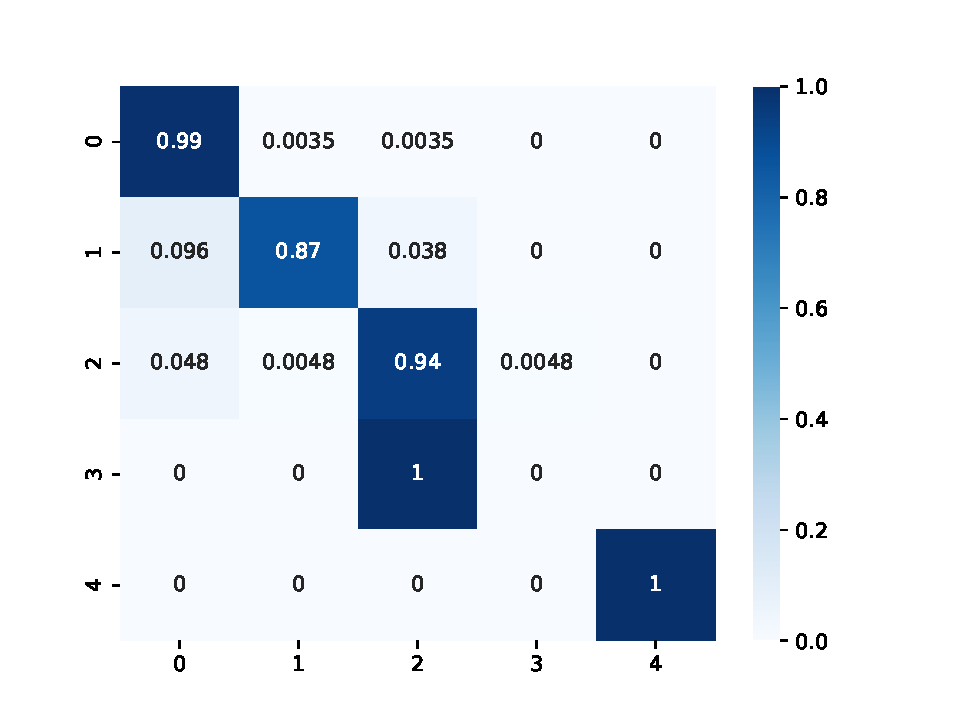
\includegraphics[keepaspectratio, scale=0.6]{images/deep_conv_heatmap.pdf}
      \label{fig:heatmap_ratio}
    \end{figure}
  \end{frame}

  \begin{frame}{混同行列(個数)のヒートマップ\footnote{縦軸が正解ラベル、横軸が予測ラベル}}
    \begin{figure}
      \centering
      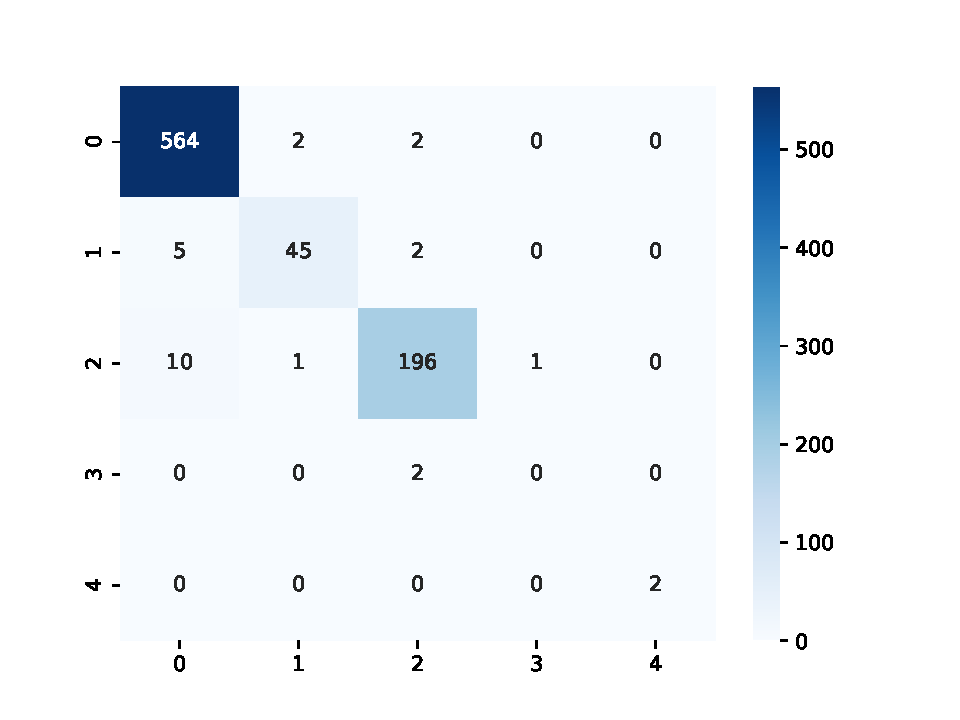
\includegraphics[keepaspectratio, scale=0.6]{images/deep_conv_cnt_heatmap.pdf}
      \label{fig:heatmap_cnt}
    \end{figure}
  \end{frame}

  \begin{frame}{考察}
    \begin{itemize}
      \item メモリが数値でわかりにくいので、ファミリー名で表す
      \item x軸とy軸のラベルを入れる
      \item 正解ラベルが1または2で、予測ラベルが0となって間違っているデータが多い \mbox{}\\ $\rightarrow$データの偏りが原因として考えられるので、水増しをしたら正解率上がるかも
    \end{itemize}
  \end{frame}

  \begin{frame}
    \section{まとめ}
  \end{frame}

  \begin{frame}{まとめ}
    \begin{itemize}
      \item k分割交差検証をsklearnを用いて訓練データと検証データのラベルの比率を9:1に揃える
      \item 混同行列のヒートマップのラベルをファミリー名に直す
      \item 卒論を書く
    \end{itemize}
  \end{frame}
\end{document}


